\documentclass[letterpaper, reqno,11pt]{article}
\usepackage[margin=1.0in]{geometry}
\usepackage{color,latexsym,amsmath,amssymb,graphicx,float,listings,tikz}
\usepackage{hyperref}

\hypersetup{
colorlinks=true,
linkcolor=magenta,
filecolor=magenta,
urlcolor=cyan,
}

\graphicspath{ {images/} }

\begin{document}
\pagenumbering{arabic}
\title{Math 318 Homework 5}
\date{02/03/23}
\author{Xander Naumenko}
\maketitle

% {\medskip\noindent\bf Question 1a.} The CDF $F_M$ at a point $x$ is the probability that each of the $X_i$ variables is greater than $x$, which happens with probability $1-x$. 

% \[
% F_M(x) = \int_0^{x}x'(1-x')^{n}dx'
% .\]

{\medskip\noindent\bf Question 1a.} The meaning of $1-F_M(x)$ is the probability that the minimum is above a given value $x$. This occurs when each of the $X_i$ are above $x$, which happens with probability each $1-x$. Thus we have 
\[
1-F_M(x)=(1-x)^{n}\implies F_M(x)=\begin{cases}
    1&\text{if }x\leq 0\\
    1-(1-x)^{n} &\text{if } 0\leq x\leq 1\\
    0&\text{if }x\geq 1
\end{cases} 
.\]

{\medskip\noindent\bf Question 1b.} The PDF is just the derivative of the CDF: 

\[
f_M(x)=\frac{d}{dx}F_M(x)=n(1-x)^{n-1}1_{0\leq x\leq 1}
.\]

{\medskip\noindent\bf Question 1c.} To find the mean we can integrate: 
\[
    \mu=\int_0^{1}nx(1-x)^{n-1}dx=x(1-x)^{n}\bigg|_0^1+\int_0^{1}(1-x)^{n}dx=\frac{1}{n+1}
.\]
Similarly for the variance, omitting the boundary terms since as in the previous calculation they obviously go to zero: 
\[
    \text{Var}(M)=\int_0^{1}nx^2(1-x)^{n-1}dx -\frac{1}{(n+1)^2}=\int_0^{1}2x(1-x)^{n}dx-\frac{1}{(n+1)^2}=\int_0^{1}\frac{2}{n+1}(1-x)^{n+1}dx-\frac{1}{(n+1)^2}
\]
\[
=\frac{2}{(n+1)(n+2)}-\frac{1}{(n+1)^2}
.\]

{\medskip\noindent\bf Question 1d.} Let $y=xn$. Then the CDF of $Y$ is 
\[
F_Y(y)=F_M(\frac{y}{n})=1-(1-\frac{y}{n})^{n}
.\]
\[
    f_Y(y)=\frac{d}{dy}F_Y(y)=(1-\frac{y}{n})^{n-1}1_{0\leq y\leq n}
.\]

{\medskip\noindent\bf Question 1e.} Taking the limit and using a definition of $e$ stated in class:

\[
\lim_{n\to\infty}=(1-\frac{y}{n})(1-\frac{y}{n})^{n}=\lim_{n\to\infty}(1-\frac{y}{n})e^{-y}=e^{-y}
.\]

{\medskip\noindent\bf Question 2.} Clearly $E[X]=0.5$ and $E[Y]=-0.5$ since they're uniform distributions. We also have
\[
    E[X^2]=E[Y^2]=\int_0^{1}x^2dx=\frac{1}{3}
.\]
% Also the CDF of $X^2$ is $P(X^2<x)=P(X<\sqrt{x} )=\sqrt{x}$, so the PDF is $f_{X^2}(x)=\frac{1}{2\sqrt{x} }$. A similar calculation for $Y^2$ shows that $f_{Y^2}(y)=\frac{1}{2\sqrt{-y} }$. 

Now computing the covariance using the definition
\[
    \text{cov}(X, X^2)=E\left[(X-E[X])(X^2-E[X^2])\right]=E[XX^2]-E[X]E[X^2]%\int_0^{1}x(x-\frac{1}{2})(x^2-\frac{1}{3})dx
\]
\[
    =\int_0^{1}x \frac{d}{dx'}P(X^3<x')dx-\frac{1}{6}=\int_0^{1}\frac{1}{3}x^{\frac{1}{3}}dx-\frac{1}{6}=\frac{1}{4}-\frac{1}{6}=\frac{1}{12}
.\]
Doing the same calculation for $Y$: 
\[
    \text{cov}(Y, Y^2)=E\left[(Y-E[Y])(Y^2-E[Y^2])\right]=E[YY^2]-E[Y]E[Y^2]%\int_0^{1}x(x-\frac{1}{2})(x^2-\frac{1}{3})x
.\]

\[
    =\int_{-1}^{0}\frac{1}{3}y y^{\frac{-2}{3}}dy-\frac{1}{6}=-\frac{1}{4}-\frac{1}{6}=-\frac{1}{12}
.\]

{\medskip\noindent\bf Question 3a.} Note that $x=\frac{1}{2}\left( u+v \right) $ and $y=\frac{1}{2}\left( u-v \right) $. Computing the Jacobian: 
\[
    J(x,y)=\begin{vmatrix}\frac{\partial \frac{u+v}{2}}{\partial u} & \frac{\partial \frac{u+v}{2}}{\partial v}\\\frac{\partial \frac{u-v}{2}}{\partial u} & \frac{\partial \frac{u-v}{2}}{\partial v}\\\end{vmatrix}=\frac{1}{4}\begin{vmatrix}1&1\\1&-1\end{vmatrix}=\frac{1}{2}
.\]

Thus we have that
\[
f_{U,V}(u,v)=f_{X,Y}(\frac{1}{2}(u+v),\frac{1}{2}(u-v)) J(x,y)=\frac{1}{2\pi}e^{-\frac{1}{4}\left((u+v)^2-(u-v)^2\right)}=\frac{1}{4\pi}e^{-\frac{1}{4}\left( u^2+v^2 \right) }
.\]

{\medskip\noindent\bf Question 3b.} Consider the characteristic functions of $U$ and $V$. Then we have 
\[
    \phi_U(t)=\phi_{X+Y}(t)=\phi_X(t)\phi_Y(t)=e^{-t^2}\implies f_U(u)=\frac{1}{2\sqrt{\pi }}e^{-\frac{1}{4}u^2}
.\]

A similar calculation for $V$:
\[
    \phi_V(t)=\phi_{X-Y}(t)=\phi_X(t)\phi_{-Y}(t)=e^{-t^2}\implies f_V(v)=\frac{1}{2\sqrt{\pi}}e^{-\frac{1}{4}v^2}
.\]
Therefore we have that 
\[
f_U(u)f_V(v)=\frac{1}{4\pi}e^{-\frac{1}{4}\left(u^2+v^2\right)}
.\]
Since is the same as our result from 3a, they are independent.

{\medskip\noindent\bf Question 3c.} We already calculated the marginal distribution in part b using the characteristic functions, where we found it to be
\[
f_U(u)=\frac{1}{2\sqrt{\pi} }e^{-\frac{1}{4}u^2}=N(0,2)
.\]

{\medskip\noindent\bf Question 4a.} Integrating to find the marginal distribution:
\[
f(x)=\int_0^{\infty}\lambda^2e^{-\lambda z}1_{0\leq x\leq z}dz=\int_x^{\infty}\lambda^2e^{-\lambda z}dz=\lambda e^{-\lambda x}1_{0\leq x}
.\]

{\medskip\noindent\bf Question 4b.} Doing same as previous question: 
\[
f(z)=\int_0^{\infty}\lambda^2e^{-\lambda z}1_{0\leq x\leq z}dx=\int_0^{z}\lambda^2e^{-\lambda z}dx=\lambda^2z e^{-\lambda z}1_{0\leq z}
.\]

{\medskip\noindent\bf Question 4c.} As the hint suggests, we can take the derivative of the joint cumulative distribution function of $X$ and $Y$. To find what this is, we can first find the joint cumulative distribution of $X,Z$: 
\[
F_{X,Z}(x,z)=\int_0^{z}\int_0^{x}\lambda^2e^{-\lambda z'}1_{0\leq x'\leq z'}dx'dz'=\int_0^{z}\lambda^2e^{-\lambda z'}\min(x,z')dz'
\]
\[
=\int_0^{x}\lambda^2z' e^{-\lambda z'}dz'+x\int_x^{z}\lambda^2e^{-\lambda z'}dz'=-\lambda z'e^{-\lambda z'}\bigg|_0^x+\int_0^x\lambda e^{-\lambda z'}dz'+\lambda xe^{-\lambda x}-\lambda x e^{-\lambda z}
.\]
\[
=1-e^{-\lambda x}-\lambda xe^{-\lambda z}
.\]
We can then do the calculation to find the joint density
\[
f_{X,Y}(x,y)=\frac{d}{dx}\frac{d}{dy}P(X\leq x,Y\leq y)=\frac{d}{dx}\frac{d}{dy}P(X\leq x, Z\leq x+y)=\frac{d}{dx}\frac{d}{dy}F_{X,Z}(x,x+y)
\]
\[
=\frac{d}{dx}\frac{d}{dy}\left( 1-e^{-\lambda x}-\lambda e^{-\lambda (x+y)} \right) =\frac{d}{dx}\lambda^2 e^{-\lambda(x+y)} 
\]
\[
=\lambda ^2e^{-\lambda(x+y)}1_{0\leq x\leq z}
.\]

{\medskip\noindent\bf Question 4d.} Finding the marginal pdf: 
\[
f_Y(y)=\int_0^{\infty}\lambda^2e^{-\lambda(x+y)}dx=\lambda e^{-\lambda y}
.\]

{\medskip\noindent\bf Question 5a.} The following python code was used to produce the output. The result was $P(A)\approx 0.0271$. 

\begin{lstlisting}[language=Python]
from math import comb
n = 100
p = 0.6
P = sum([comb(n, k) * p**k * (1-p)**(n-k) for k in range(0, 51)])
print(P)
\end{lstlisting}

{\medskip\noindent\bf Question 5b.} Let $X_1, X_2,\ldots, X_{100}$ be a set of independent Bernoulli variables with parameter $p=0.6$, so $X=\sum_{i=1}^{100}X_i$. The mean of $X$ is clearly $np=60$ and the variance of each $X_i$ is $0.6\cdot 0.4=0.24$, so by the central limit theorem we have 
\[
Z=\frac{X-60}{\sqrt{24} }\approx N(0,1)
.\]

{\medskip\noindent\bf Question 5c.} Using the fact that $X=\sqrt{24} Z+60$, we get: 
\[
P(X\leq 50)= P(\sqrt{24} Z+60\leq 50)=P(Z\leq -\frac{10}{\sqrt{24} })\approx \Phi(-\frac{10}{\sqrt{24} })\approx 0.0206
.\]

{\medskip\noindent\bf Question 5d.} Using the exact same approach as part c except with 51 instead of 50: 
\[
P(X< 51)= P(\sqrt{24} Z+60< 51)=P(Z<-\frac{9}{\sqrt{24} })\approx \Phi(-\frac{9}{\sqrt{24} })\approx 0.0331
.\]

{\medskip\noindent\bf Question 5e.} Taking the pattern from parts c and d, we get that 
\[
P(X< 50.5)= P(\sqrt{24} Z+60< 50.5)=P(Z<-\frac{9.5}{\sqrt{24} })\approx \Phi(-\frac{9.5}{\sqrt{24} })\approx 0.0262
.\]

{\medskip\noindent\bf Question 6a.} We can compute the probability distribution of each $S_n$ by taking convolutions of the pdfs of $S_{n-1}$ $X_n$. The following code does this, the resultant graphs can be seen in figure \ref{fig:6a}

\begin{lstlisting}[language=Python]
import numpy as np
import matplotlib.pyplot as plt
from scipy.stats import norm

ns = (1,2,3,4,5,10,50)

u = np.array([1/3, 1/3, 1/3])
S = [u]

for i in range(1, max(ns)+1):
    s = np.convolve(u, S[-1])
    S.append(s)

fig,ax = plt.subplots(nrows=4, ncols=2, sharey=True)
for i,n in enumerate(ns):
    a = ax[i//2,i%2]
    a.plot(S[n-1], label='$S_n$')
    a.title.set_text(f'n={n}')
    mu = n
    var = 2/3 * (n)
    
    x = np.arange(len(S[n-1]))
    a.plot(norm.pdf(x, mu, var**0.5), label=f'$N({mu},{round(var,1)})$')
    a.legend()

plt.show()
\end{lstlisting}

\begin{figure}[htpb]
    \centering
    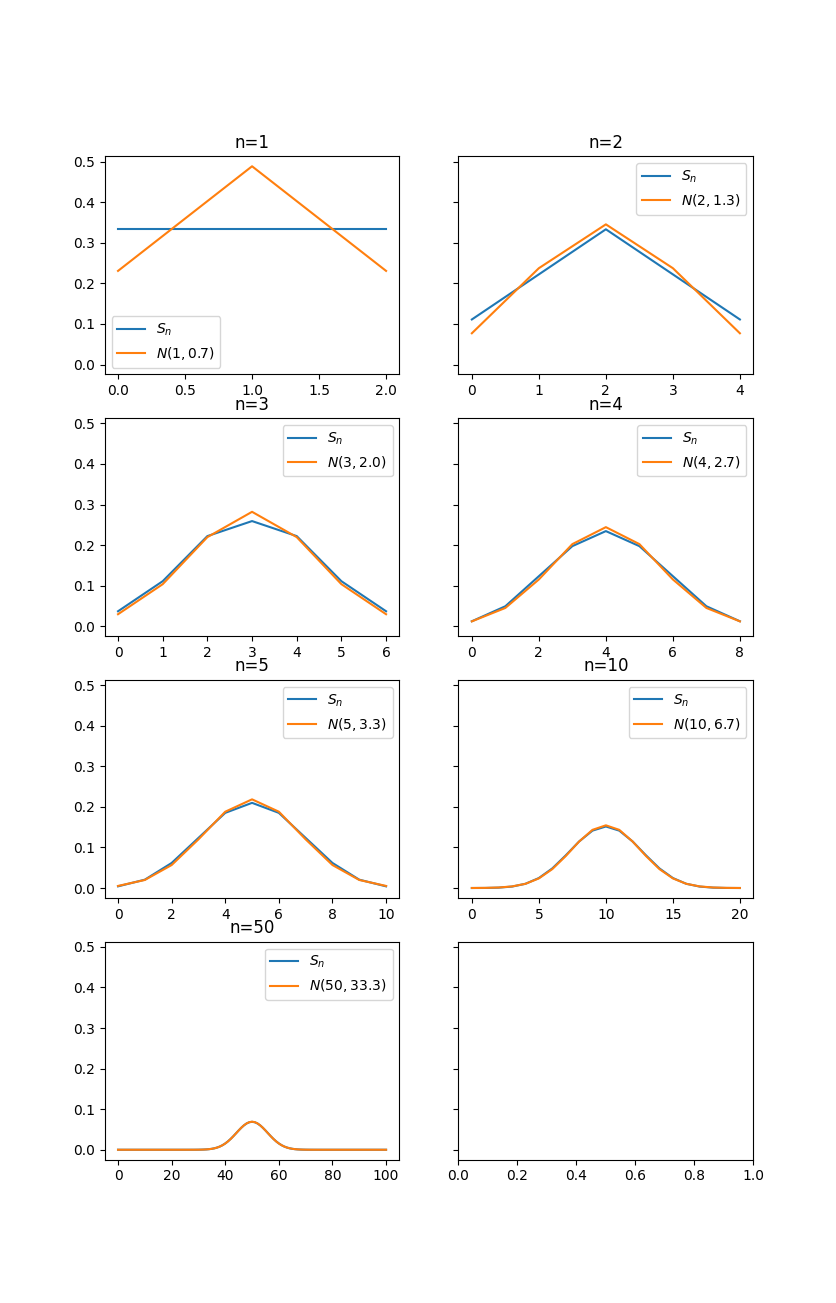
\includegraphics[width=0.8\textwidth]{6a}
    \caption{Graphs for question 6a}
    \label{fig:6a}
\end{figure}

{\medskip\noindent\bf Question 6b.} The resulting plots can be seen in figure \ref{fig:6b}. The code very similar to the previous part, it is as follows: 

\begin{lstlisting}[language=Python]
import numpy as np
import matplotlib.pyplot as plt
from scipy.stats import norm

ns = (1,2,3,4,5,10,50)

x = np.array([-1, 0, 1, 2, 3, 4])
y = np.array([1/15, 1/15, 11/15, 1/15, 0, 1/15])
X = [x]
T = [y]

for i in range(1, max(ns)+1):
    first = X[-1][0]
    last = X[-1][-1]
    X.append(np.insert(np.append(X[-1], [last+1, last+2, last+3, last+4])\
        , 0, first-1))
    T.append(np.convolve(y, T[-1]))

fig,ax = plt.subplots(nrows=4, ncols=2, sharey=True)
for i,n in enumerate(ns):
    a = ax[i//2,i%2]
    a.plot(X[n-1], T[n-1], label='$S_n$')
    a.title.set_text(f'n={n}')
    x = X[n-1]
    t = T[n-1]
    mu = sum([x[i] * y for i,y in enumerate(t)])
    var = sum([(x[i]-mu)**2 * y for i,y in enumerate(t)])
    
    a.plot(X[n-1], norm.pdf(X[n-1], mu, var**0.5), label=f'$N({mu},{round(var,1)})$')
    a.legend()

plt.tight_layout()
plt.show()


\end{lstlisting}

\begin{figure}[htpb]
    \centering
    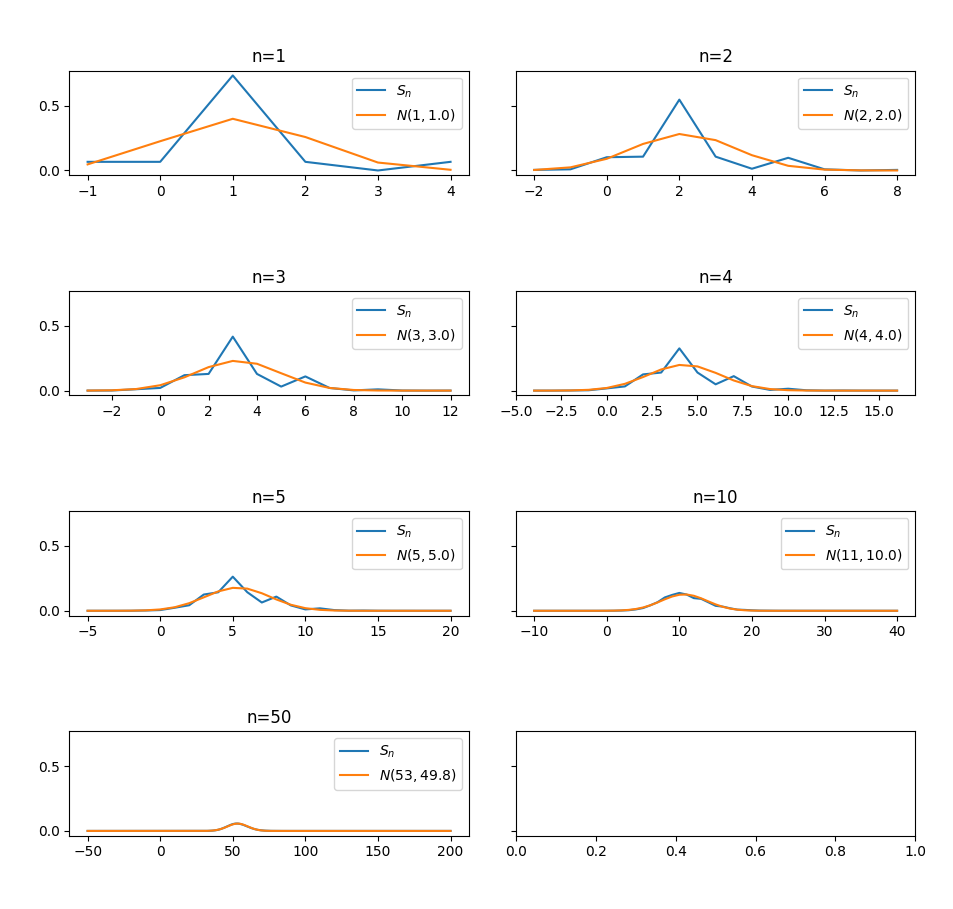
\includegraphics[width=0.8\textwidth]{6b}
    \caption{Graphs for 6b.}
    \label{fig:6b}
\end{figure}


\end{document}
